\section{Introduction}
%\pmcomment{Show that you can do this on different types of datasets. Verifair only runs on simulated datasets - compared to our results on a broad class of datatypes.}

%\pmcomment{One pass over introduction completed}

%\pmcomment{Currently working on merging introduction and related work}

The use of advanced analytics and artificial intelligence (AI), along with its many benefits, poses important threats to individuals and the broader society at large.
%\pmcomment{SRINI - I think it is ok - its been out for a couple of years and has a few cites already. Pranav - We may need another reference in addition to this for anonymity}
\cite{hirsch20corporate} identify invasion of privacy; manipulation of vulnerabilities;  bias against protected classes; increased power imbalances;  error; opacity and procedural unfairness; displacement of labor;  pressure to conform, and intentional and harmful use as some of the key areas of concern.
A core part of the solution %space
to mitigate such risks is the need to make organizations accountable and ensure that the data they leverage and the models they build and use 
are both inclusive of marginalized groups and resilient against societal bias.
Deployed AI and analytic systems are complex multi-step processes that can produce several sources of risk at each step.
%\begin{leftbar}
At each of these stages, determining accountability in the decision-making in AI processes requires a determination of who is accountable, for what, to whom, and under what circumstances~\citep{nissenbaum1996accountability,cooper2022accountability}. 
\todo{Contextualizing wrt Nissenbaum}
%\marginpar[]{}
A more comprehensive overview of the mechanisms that can support accountability with respect to the different stages of design of a machine learning system can be found in the work of \citet{cooper2022accountability}.
%\end{leftbar}
We center our analysis on the sub-problem of auditing barriers towards investigating claims surrounding mathematical guarantees of automated decision making processes.
Governments across the world are wrestling with the implementation of auditing regulation and practices for increasing the accountability of decision processes.
Recent examples include the New York City auditing requirements for AI hiring tools~\citep{vanderford2022nybiaslaw}, European data regulation (GDPR~\citeyear{GDPR}), accountability bills~\citeyear{congress2019hr,algtransparency2022} and judicial reports~\citeyear{justice2018free}.
%In an evolving environment, organizations also aim to augment their understanding of algorithmic audits.
These societal forces have led to the emergence of checklists~\citep{mitchell2019model,sokol2020explainability}, metrics of fairness~\citep{verma2018fairness}, and recently, algorithms and systems that observe and audits the behavior of %advanced analytics and
AI algorithms.  %We note that 
Such ideas date back to the 1950s~\citep{moore1956gedanken} % for black box automata), 
but research has largely been sporadic until very recently with the widespread use of AI-based decision making giving rise to the vision of algorithmic auditing~\citep{clavell2020auditing}.
We present a framework for {\it Auditing and Verifying fairness Online through Interactive Refinement}~(\AVOIRmethodname{})
\footnote{AVOIR in French means ``to have'' and this acronym reflects both our aspirational goal to achieve fairness in advanced analytics and AI but also reflects what is currently verifiable given a dataset, a model and a fairness specification.}.
\AVOIRmethodname{} builds upon the ideas on distributional probabilistic fairness guarantees~\citep{albarghouthi2019fairness,bastani2019probabilistic}, generalizing them to real-world data. 
An overview of \AVOIRmethodname{} is provided in Figure~\ref{fig:framework}.
%Delivering on this vision would allow organizations and regulators to gain some understanding on whether the algorithmic decision-making models they are using are verifiably meeting regulatory standards.
%Such ideas are  essential to building trust in service platforms and facilitate platform regulation. 
%Importantly such ideas are needed both at the data and  algorithmic  level - mirroring recent regulatory advances.
%Despite their ubiquitous use, biases from the labeled data or algorithm design can arise and raise concerns about machine learning decisions.
%Further, some applications require decision-making processes to follow regulatory frameworks.

\begin{figure}[ht]
    \centering
    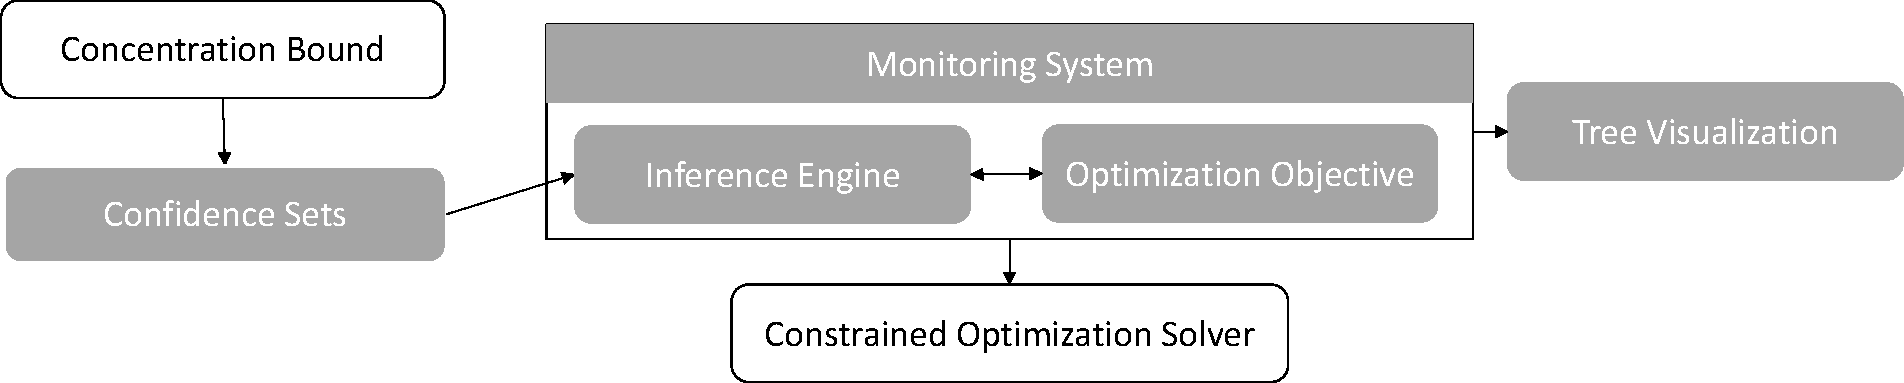
\includegraphics[width=0.7\linewidth]{avoir/images/Framework.pdf}
    \caption{Shaded nodes describe our contributions in the \AVOIRmethodname{} framework.}
    \label{fig:framework}
\end{figure}

\subsection{Preliminaries}
Machine learning testing~\citep{zhang2020mltesting} is an avenue that can be used to expose undesired behavior and improve the trustworthiness of machine learning systems.
%Testing in software systems relies on assertions over the behavior of the functions being tested.
Fairness criteria quantify the relationship between the outcome metric across multiple subgroups or similar individuals among the population.
Formal definitions of fairness focus on observational criteria, i.e., those that can be written down as a probability statement involving the joint distribution of the features, sensitive attributes, decision making function, and actual outcome. %from https://fairmlclass.github.io/4.html#/2
Our framework, \AVOIRmethodname{}, supports implementing a large range of group fairness criteria, including demographic parity~\citep{calders2009building}, equal opportunity~\citep{hardt2016equality}, disparate mistreatment~\citep{zafar2017fairness}, and various combinations of these criteria. 
%We give an example of a fairness metric and the corresponding fairness specification here.
%For example, a decision making function that selects amongst applicants to hire for a specific position may have different hiring rates for majority and minority population groups. 
As an example, suppose $r \in \{ 0, 1\}$ denotes the return value of a binary decision function (say, candidate selection for a job), and $s$ is an indicator denoting whether a candidate belongs to a minority population.
The 80\%-rule for disparate impact~\citep{eeoc1979,feldman2015certifying} is a fairness criterion which states that
\begin{align*}
    \frac{\Pr[r=1| s]}{\Pr[r=1| \neg s]} \geq 0.8 
\end{align*}
\todo{Section to introduce the terms.}
%Decision making/scoring functions aim to optimize for a specific metric such as accuracy, precision, F1 score etc. 
%Fairness criteria, on the other hand, quantify the relationship between the outcome metric across multiple subgroups or similar individuals among the population. 
When implemented in the \AVOIRmethodname{} DSL grammar, the above 80\%-rule would be the specification \lstinline{E[r|S==s] / E[r|S!= s] >= 0.8}.
Here, the term \lstinline{E[r|S!=s]/E[r|S == s]} is a \textit{subexpression} of the specification.
The smallest units involving an expectation (eg., \lstinline{E[r|S!=s]}) are denoted as an \textit{elementary subexpressions}.
Our algorithm works by using adaptive concentration sets~\citep{zhao2016adaptive,howard2021time} to build estimates for \textit{elementary subexpressions}, and then deriving the estimates for expressions that combine them.
We aim to derive statistical guarantees about fairness criteria based on estimates from observed outputs.
For example, let $X$ be an observed Bernoulli r.v\footnote{random variable}, then an assertion $\phi_X = (\BarE[X], \epsilon, \delta)$ over $X$, corresponds to an estimate satisfying
\begin{equation}\label{eqn:eps-delta-defn}
  \phi_X \equiv \Pr[|\E[X] - \BarE[X]| \geq \epsilon] \leq \delta  
\end{equation}
where $\BarE[X]$ denotes an empirical estimate of $E[X]$.
We then use assertions $\phi_X, \phi_Y$ to assert claims for expressions involving $X, Y$.
For example, for the 80\%-rule, assertions over $X/Y$.
A specification involves either a comparison of expressions with constants (eg., $X/Y > 0.8$), or a combination of multiple such comparisons. 
Such a specification may be True ($T$) or False ($F$) with some probability.
For a given specification $\psi$, we denote the claim that $P[\psi = F] \geq 1 - \delta$ as $\psi: (F, \delta)$, where $\delta$ denotes the failure probability of a guarantee. 
Given a stream of (observations, outcomes from the decision functions), and a specified threshold probability $\delta$, we will continue to refine the estimate for a given specification until we reach the threshold.
We focus on fairness criteria that can be expressed using Bernoulli r.v. as it allows the simplification of probabilities into expectation, as $\Pr[r = 1] = \E[r]$.
Specifications involving variables that take more than two values can be implemented using transformations and boolean operators (examples in Appendix~\ref{sec:appendix:additional-metrics}).
%\pmcomment{Discussion of Individual vs Group fairness here?}
%Section~\ref{sec:casestudy} contains descriptive analyses and case studies of real world applications of \AVOIRmethodname{} on commonly used fairness criteria.
%\pmcomment{more about fairness criteria group fairness etc?}

%\subsection{Fairness Specifications}
%The method will terminate when the specification can be asserted as being either True or False with a likelihood $> 1 - \delta$.
%\pmcomment{We can use $\HatMu_X$ instead of $\BarE[X]$ - does it look cleaner?}